% !TEX root = ../../I4PRJ, Grp3 - Rapport.tex
\chapter{Proces og projektgennemførsel}

I afsnittet beskrives projektgennemførelsen og proces. Herunder udviklingmetode, processtyring, ledelse og værktøjer.

\section{Proces}
Udviklingsmetoden for projektet er Scrum. Scrum er en agil udviklingsmetode \cite[kap. 1]{robertmartin2006}. Scrum er ikke indlemmet i processen i sin kanoniske form. I næste afsnit beskrives, hvordan projektprocessen afviger fra teorien.

\section{Scrum}
Scrum sprints har været forlænget. Da Scrum typisk bruges i fuldtids-udviklingteams\todo{reference}, kunne det ikke lade sig gøre at have nok at samle op på efter en uges arbejde. Daglige Scrum meetings er blevet til ugentlige. Spørgsmålene: Hvad har jeg lavet? Hvad mangler jeg at lave? Hvad skal der til, for at jeg kommer videre?, er blevet besvaret af hvert gruppemedlem. Den forlængede tid mellem møder har medført at sprints har strukket sig over 2-3 uger af gangen. Med Scrum har gruppen forsøgt at være refleksiv over processen. Hvor spørgsmålene stilles; Hvad skal vi blive ved med at gøre? Hvad skal vi holde op med at gøre? Hvad skal vi begynde at gøre? På samme måde har gruppen reflekteret over processen og har eksempelvis løst følgende misforståelse og gjort gruppen opmærksom på øget kommunikation:

Der var gruppemedlemmer, som havde tendens til at arbejde på en del af systemet, uden at der var åbenhed omkring det. Det kunne have ført til evt. dobbeltarbejde, som ville have været spildt. Problemet blev bragt op tidligt i processen, hvormed gruppen har indgået konsensus om åbenhed af arbejdsopgaver, hvilket har gjort det nemmere at koordinere arbejde på tværs af undergrupper.

Gruppen har ikke anvendt den traditionelle rollefordeling i et Scrumteam. Alle gruppens medlemmer har været ligestillet som udviklere og rollerne som Scrum master og product owner har været en diskussion på møder, hvor demokratiske beslutninger er foretaget som erstatning. Til alle møder er der taget referat, og referent rollen er blevet udtrukket ved et hertil udviklet værktøj. Til alle møder er der blevet valgt en mødeleder. Mødelederens rolle var ordstyrer og ansvar for overholdelse af dagsorden.

For at holde styr på status i processen og i de enkelte sprints opererer Scrum med backlogs. Det er product backlog og sprint backlog, som i projektet er oprettet ved hjælp af værktøjet "Pivotal Tracker". 

\subsection{Pivotal Tracker}
Pivotal Tracker \url{pivotaltracker.com/} er et processtyringsværktøj, til projekter som bruger Scrum som udviklingsmetode. De forskellige backlogs i et Scrum projekt opstilles nemt og intuitiv i Pivotal. Pivotal benytter story begrebet, hvilket har gjort det nemt at arbejde med user stories og manøvrere user stories mellem stadier af udfærdigelse. Figur~\ref{fig:scrumboard} viser et eksempel på gruppens Pivotal Tracker side.

\todo{Flyt figuren til dokumentation}
\begin{figure}
	\centering
	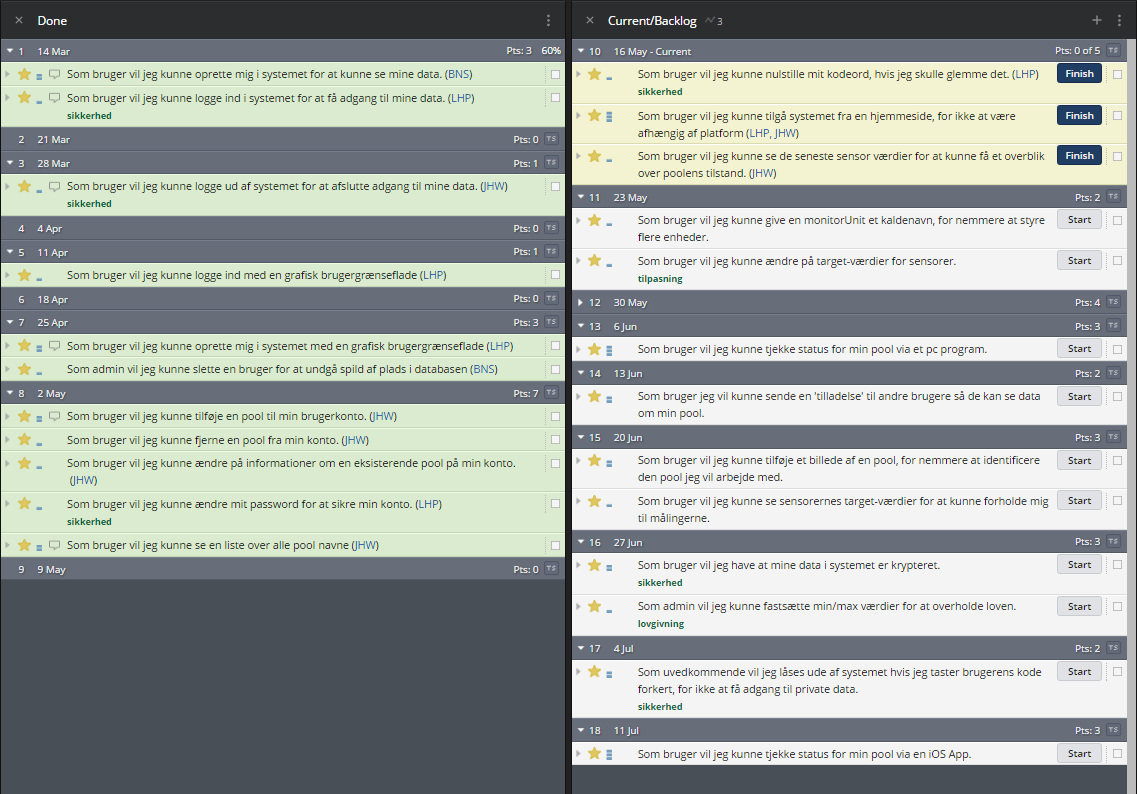
\includegraphics[width=\linewidth]{figs/processProjektGennemforsel/scrumboard.PNG}
	\caption{Pivotal tracker's interaktive scrumboard}
	\label{fig:scrumboard}
\end{figure}

 User stories er meget generelle og forklarer slutbrugers perspektiv. Det var en hjælp for gruppen at dele user stories op i mindre tasks - typisk specifik til den respektive undergruppes arbejde. 
%
%\begin{figure}
%	\centering
%	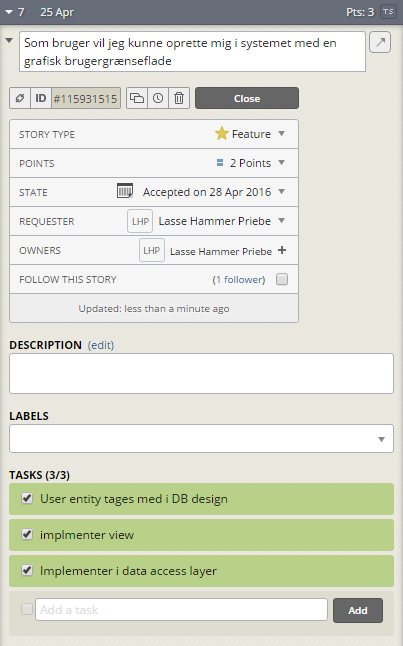
\includegraphics[width=0.4\linewidth]{figs/processProjektGennemforsel/userstory_with_tasks.PNG}
%	\caption{User Story - Opret Bruger}
%	\label{fig:userstory_with_tasks}
%\end{figure}

%Som det ses på figur~\ref{fig:userstory_with_tasks} giver Pivotal Tracker mulighed for at tjekke tasks af efterhånden som de udføres. Når alle tasks i den pågældende user story er tjekket, så trykkes Deliver, herefter kan en ny story påbegyndes. 

Start af nye user stories eller tasks sker ved et scrum møde. For at sikre at arbejdsbyrden er passende for sprintet, vurderes hver user story af alle medlemmer. Hver user story vurderes på en skala fra 1-3. Efter hvert sprint opgøres det, hvor mange point gruppen har lavet i løbet af sprintet. Gruppens hastighed er lig med antallet af point. Ved planlægning af et nyt sprint vurderes det, om gruppen kan arbejde med samme hastighed, hvorefter arbejdsbyrden planlægges. User stories som giver meget værdi for kunden udvælges først.  

\section{Test}
Sidste led i udviklingen af en del-feature er test. Det gælder for alle lag af projektet, dog adskiller måden at teste sig i de forskellige lag. GUI blev testet ved en kvalitativ test af en udvikler. Til Business logikken er klassernes metoder unit testet. Grundet MVP strukturen i applikationslaget kan præsentationslogikken testes. Det får derfor ikke afgørende betydning at GUI er svær at teste. Databasen er testet ved unit test, hvor der testes op imod en lokal database.  

Software testing har været en stor del af dette projekt. Der har været stor fokus på robusthed. Der er i alt skrevet lidt over 200 automatiserede tests, hvilket er beskrevet nærmere i dokumentationen. Af disse er lidt over halvdelen skrevet til Data Access Layer, da eksempelvis GUI laget hovedsageligt er testet visuelt.

\subsection{Test Driven Development}
TDD er en udviklingsmetode, som foreskriver at test skrives før selve produktionskoden \cite{osherove2015art}. Gruppen har ikke brugt TDD 100\% gennem forløbet. 
Dog har TDD været særligt brugbart i udviklingen af DAL\footnote{Data Access Layer} , idet de enkelte methoder har været enkle nok, til der kunne skrives test før selve produktionskoden skulle skrives.

\subsection{Spike} 
Spike blev brugt til at teste login funktionaliteten fra ende til anden af systemet. Brugeren logger ind gennem et GUI, hvorefter systemet forespørger database om brugeren eksisterer, og slutteligt bekræftes det, at brugeren er logget ind. Integration af systemet er foretaget løbene. Det er gjort for hele tiden at teste, om arbejdet er på vej i den rigtige retning. 

\begin{figure}
	\centering
	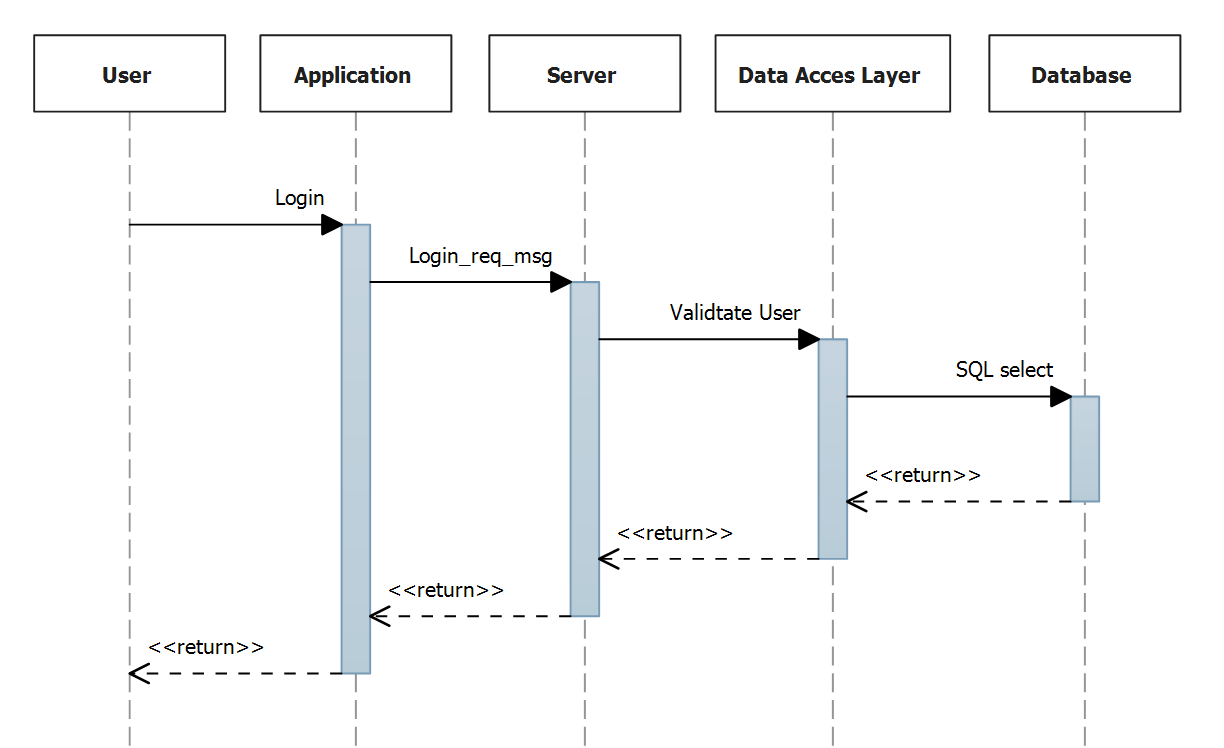
\includegraphics[width=0.8\linewidth]{figs/processProjektGennemforsel/Spike.PNG}
	\caption{Design Spike}
	\label{fig:design_spike}
\end{figure}

\section{Versionsstyring}
Softwareudviklingen er versionsstyret, for at flere udviklere kan arbejde parallelt på et projekt uden at skabe konflikter når ændringer gemmes. Til formålet har gruppen benyttet Git.

\subsection{Git}
Git bruges i projektet til deling og versionsstyring af al source kode.
For at holde styr på branches og versioner er der brugt Feature Branching \cite{atlassian2016}. Det indebære, at der ikke foregår noget produktionsarbejde på master branchen. I stedet skal der oprettes en branch specielt til hver feature. Når denne feature er testet med seneste udgave af master branchen, kan ændringerne blive "merged" eller flettet ind. På denne måde har gruppen hele tiden haft et fungerende produkt.

\subsubsection{GitHub}
Github er online hosting af Git repositories, og er brugt i projektet til at gemme source kode, samt administrere projektets repository. Github har været brugt til eksempelvis at tracke teamets effektivitet og commit-frekvens.

\subsection{Travis CI og Jenkins} 
Gruppen har undervejs forsøgt sig med både Travis CI og Jenkins. Travis er væsentlig bedre til at integrere med Github, så det er valgt til projektet.
Begge værktøjer er til continuos integration. CI er belejligt idet en ekstern server står for at bygge al source kode, der bliver pushet til projektets repository og kører tilsvarende tests.

Det er især nyttigt til større projekter, hvor lokale test på udviklerens computer ikke er hensigtsmæssige af tidsmæssige årsager. Travis CI er gratis til offentlige repositories på GitHub. Dog er Travis CI kun "community supported" for C\# kode \cite{communitysupportedlanguages2016}, hvilket introducerede en udfordring.

Da projektet både indeholder en applikation til PC, iOS og web, har det været en udfordring at benytte et CI-værktøj. Dette kombineret med, at hele testsuiten hurtigt kunne eksekveres lokalt, ledte til at gruppen valgte at prioritere tiden på udvikling og lokale test.

Et forsøg med Travis skulle konstatere, om der skulle bruges mere tid på Travis CI. Det lykkedes at sætte github repositoriet op til kun at tillade et merge, hvis koden kan bygge og består alle tests. Dog kunne Travis CI ikke bygge og teste med skolens database server, da denne kun kan tilgås via vpn. Det blev derfor fjernet igen.

%\begin{figure}
%\centering
%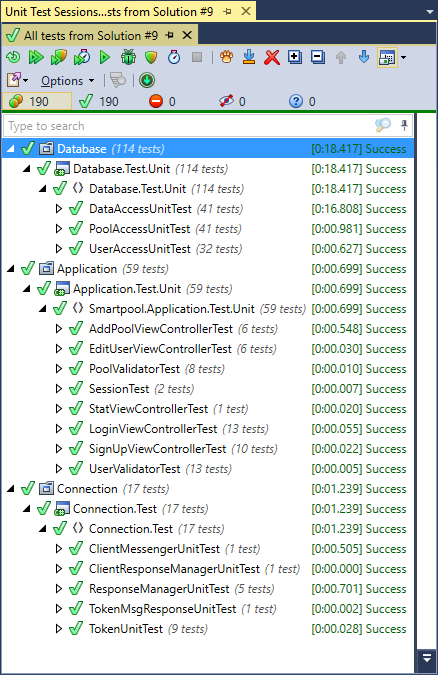
\includegraphics[width=0.6\linewidth]{figs/processProjektGennemforsel/vsUnittest.PNG}
%\caption{Samlet unittests i projektet}
%\label{fig:vsUnittest}
%\end{figure}